\subsection{Plant Characterisation}
\label{sec:sim:characterisation}

\begin{figure}[b!]
    \centering
    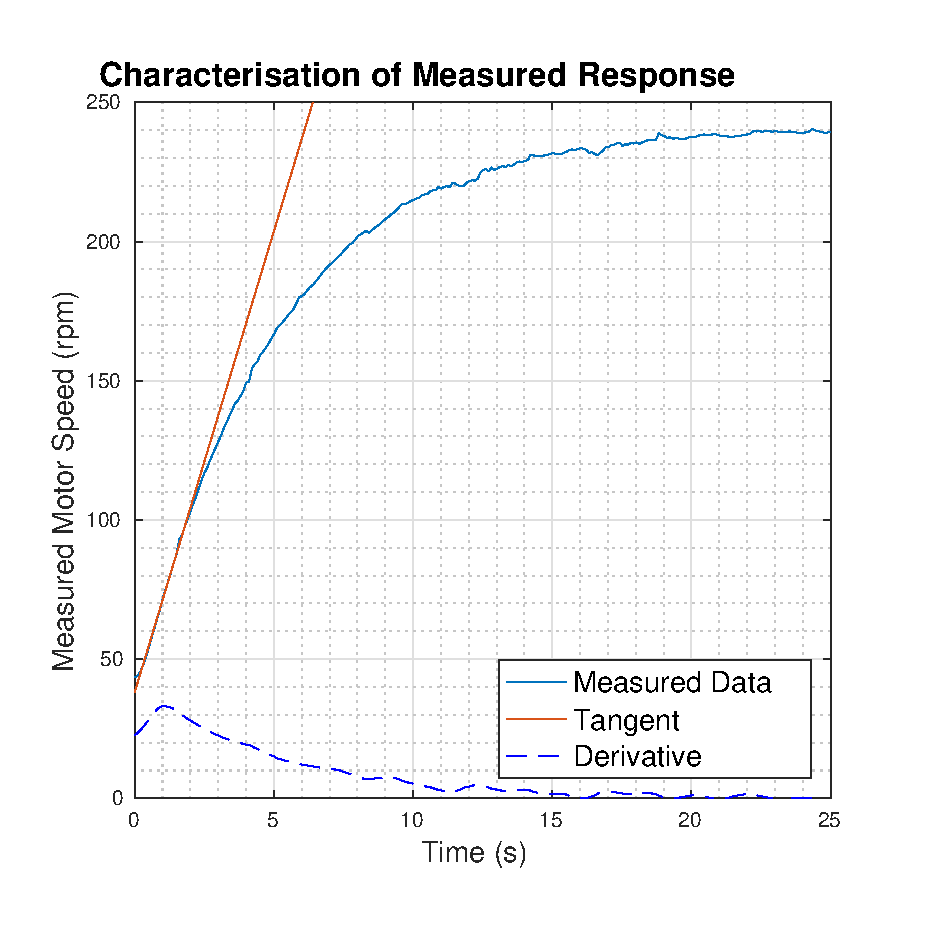
\includegraphics[width=\imagewidth]{images/characterisation}
    \caption{Calculated tangent of measured step response data.}
    \label{fig:characterisation}
\end{figure}

We decided  to  use the step response conducted in the fairly linear region of
\SI{2}{\volt}-\SI{10}{\volt} for further processing.

Using  MATLAB, the measured step  response  is  smoothed,  the  derivative  is
computed  to find the point of inflection, and the tangent is calculated.  The
results   of  this  are  visualised  in   figure   \ref{fig:characterisation}.

Regarding the parameter $K_s$, a common pitfall is to  say  that  $K_s$ is the
total  change in the step response. This  statement  is  in  fact  false,  but
happens to yield the correct value as long as the input step  function  has an
amplitude of $1$, which unfortunately is the only case studied in the majority
of theory lectures. The parameter $K_s$ is in fact the total change in  output
divided by the total change in input:

\begin{equation}
    K_s = \frac{\Delta K_{out}}{\Delta K_{in}}
\end{equation}

The calculated values of $T_u$, $T_g$ and $K_s$ turn out to be:

\begin{align*}
    T_u &= 0.1655 \\
    T_g &= 5.9602 \\
    K_s &= 197.42
\end{align*}

